\documentclass{llncs}

\usepackage{amsmath,amssymb,empheq}
\usepackage{array,bm}
%\usepackage{enumitem}
\usepackage{float}
\usepackage[T1]{fontenc}
\usepackage{graphicx}
\usepackage[utf8]{inputenc}
\usepackage{pgfplots}
\usepackage{tikz}
\usepackage{color,soul} % TODO: remove these when highlighting is no longer neccessary

\begin{document}

% TODO: Is this the final title?
\title{Assorted Load Balancing Schemes for Constrained Bin Packing Problems}

\author{
  Philippe Olivier\textsuperscript{1,2} \and
  Andrea Lodi\textsuperscript{1,2} \and
  Gilles Pesant\textsuperscript{1}}

\authorrunning{
  P. Olivier \and
  A. Lodi \and
  G. Pesant}

\institute{
  École Polytechnique de Montréal, Montreal, Canada\textsuperscript{1} \\
  CERC\textsuperscript{2} \\
  \email{\{philippe.olivier, andrea.lodi, gilles.pesant\}@polymtl.ca}
}

\maketitle

\raggedbottom
\allowdisplaybreaks


%%%%%%%%%%%%%%%%%%%%%%%%%%%%%%%%%%%%%%%%%%%%%%%%%%%%%%%%%%%%%%%%%%%%%%%%%%%%%%%%%%%%%%%%%%%%%%%%%%%%
%%%%%%%%%%%%%%%%%%%%%%%%%%%%%%%%%%%%%%%%%%%%%%%%%%%%%%%%%%%%%%%%%%%%%%%%%%%%%%%%%%%%%%%%%%%%%%%%%%%%


% Status: Pre-final
%
% TODO:
% - If we add the MH model, mention it in the abstract: "... to present and compare constraint programming, integer programming, and metaheuristic approaches."

\begin{abstract}
  Despite the existence of efficient solution methods for bin packing problems, in practice these seldom occur in such a pure form but feature instead various considerations such as pairwise conflicts or profits between items, or aiming for balanced loads amongst the bins. The Wedding Seating Problem is a combinatorial optimization problem incorporating elements of bin packing with conflicts, bin packing with profits, and load balancing. We use this representative problem to present and compare constraint programming and integer programming approaches.
\end{abstract}


%%%%%%%%%%%%%%%%%%%%%%%%%%%%%%%%%%%%%%%%%%%%%%%%%%%%%%%%%%%%%%%%%%%%%%%%%%%%%%%%%%%%%%%%%%%%%%%%%%%%
%%%%%%%%%%%%%%%%%%%%%%%%%%%%%%%%%%%%%%%%%%%%%%%%%%%%%%%%%%%%%%%%%%%%%%%%%%%%%%%%%%%%%%%%%%%%%%%%%%%%


\section{Introduction}
\label{sec:introduction}

% Status: Pre-final
%
% TODO:
% - If we add the MH model, modify to: "Sections~\ref{sec:cp_model} to~\ref{sec:mh_model} introduce, respectively, our constraint programming~(CP) model, our two integer programming~(IP) models, and our metaheuristic~(MH) model. Section~\ref{sec:benchmark_results} presents the results of our experiments."

\paragraph{}In the optimization version of the classical bin packing problem, a set of items of various weights must be packed into as few bins of limited capacities as possible. Despite the existence of efficient solution methods for bin packing problems, in practice these seldom occur in such a pure form. They instead feature various considerations such as pairwise conflicts or profits between items, or aiming for balanced loads amongst the bins. The objective then becomes to minimize some scoring function by selecting an optimal distribution of items in the available bins.

In our representative problem, the Wedding Seating Problem~(WSP) \cite{Lewis2013}, groups of guests of different sizes must be seated at tables of limited capacities. Some of these groups may or may not like each other, thus some relation is defined over each pair of them. Pairs of groups whose relation is \emph{definitely apart} can never be seated at the same table. While not strictly necessary, pairs of groups whose relation is either \emph{rather together} or \emph{rather apart} should, if possible, be seated together or apart, respectively. Pairs which have no specific relation are \emph{indifferent}. Note that an implicit relation, \emph{definitively together}, is baked into the problem as \emph{groups of guests}, the smallest indivisible entity that can be assigned to a table.

This paper is an extended and overhauled version of~\cite{Olivier2018}, which was presented at CPAIOR 2018. Section~\ref{sec:description_of_the_problem} gives a formal definition of our problem, and Sect.~\ref{sec:related_work} reviews current methods of solving the WSP and similar problems. Sections~\ref{sec:cp_model} to~\ref{sec:ip_model_b} introduce, respectively, our constraint programming~(CP) model and our two integer programming~(IP) models. Section~\ref{sec:benchmark_results} presents the results of our experiments.


%%%%%%%%%%%%%%%%%%%%%%%%%%%%%%%%%%%%%%%%%%%%%%%%%%%%%%%%%%%%%%%%%%%%%%%%%%%%%%%%%%%%%%%%%%%%%%%%%%%%
%%%%%%%%%%%%%%%%%%%%%%%%%%%%%%%%%%%%%%%%%%%%%%%%%%%%%%%%%%%%%%%%%%%%%%%%%%%%%%%%%%%%%%%%%%%%%%%%%%%%


\section{Description of the Problem}
\label{sec:description_of_the_problem}

% Status: Pre-final

\paragraph{}Let

\begin{itemize}
\item $\mathcal{I} = \{1, \dots, n\}$ be the index set of items,
\item $\mathcal{B} = \{1, \dots, m\}$ be the index set of bins,
\item $\ell$ and $u$ be, respectively, the lower and upper bounds on the load of a bin,
\item $w_{i}$ denote the weight of item $i$ with $w = \sum_{i \in \mathcal{I}} w_{i}$ representing the combined weight of all the items,
\item $c_{ij}$ the cost incurred if items $i$ and $j$ are packed into the same bin.
\end{itemize}

\paragraph{}Entries in the cost matrix $C$ can take any integer value. Namely,

\begin{equation*}
  c_{ij}
  \begin{cases}
    =\infty, & \mbox{if $i$ and $j$ are in conflict and must be packed into separate bins,} \\
    =0,      & \mbox{if $i$ and $j$ have no cost,}                                          \\
    <0,      & \mbox{if $i$ and $j$ should rather be packed into the same bin,}             \\
    >0,      & \mbox{if $i$ and $j$ should rather be packed into separate bins.}
  \end{cases}
\end{equation*}

\paragraph{}Since a conflict is expressed as being a prohibitive cost, the initial cost matrix can be enhanced by adding this prohibitive cost for each pair of items whose combined weights is greater than $u$, since they can never be packed together.

The problem consists of packing all items into the available bins such that conflicting items are packed into separate bins, under arbitrary load balancing constraints. The objective is to minimize the combined cost of all available bins. We will be considering the load balancing constraints under four distinct norms which yield incomparable results. The $L_{0}$-norm minimizes the number of values different from the mean bin load. To tackle fractional means with this norm, the two nearest integers will be considered to be within a valid mean range. The $L_{1}$- and $L_{2}$-norms minimize, respectively, the sum of absolute deviations and the sum of squared deviations from the mean. The $L_{\infty}$-norm minimizes the maximum deviation from the mean.

In order to compare the impact of the load balancing parameters, we have opted to construct a Pareto set using the $\epsilon$-constraint method~\cite{Miettinen1998}: We bounded the global deviation at successively higher intervals, each time solving the problem by minimizing the objective. We consider disjoint intervals of deviation to ensure nonoverlapping solution spaces in each step of the construction of the Pareto set, thus preventing identical solutions from being found in different steps. Parameters $d_{\min}$ and $d_{\max}$ denote the lower and upper bounds on the cumulative deviation of a solution. Presenting the parameters of the load balancing constraints with a Pareto set has the advantage of offering decision-makers multiple optimal solutions to choose from depending on their perception of the trade-offs amongst them.

\paragraph{}The problem of packing items into bins is the same as that of seating groups of guests at tables, as described by Lewis and Carroll. It has been shown to be $\mathcal{NP}$-hard as it generalizes two other $\mathcal{NP}$-hard problems: the $k$-partition problem and the graph $k$-coloring problem \cite{Lewis2016}.


%%%%%%%%%%%%%%%%%%%%%%%%%%%%%%%%%%%%%%%%%%%%%%%%%%%%%%%%%%%%%%%%%%%%%%%%%%%%%%%%%%%%%%%%%%%%%%%%%%%%
%%%%%%%%%%%%%%%%%%%%%%%%%%%%%%%%%%%%%%%%%%%%%%%%%%%%%%%%%%%%%%%%%%%%%%%%%%%%%%%%%%%%%%%%%%%%%%%%%%%%


\section{Related Work}
\label{sec:related_work}

% Status: Not started
%
% TODO:
% - Review existing methods for L0, L1, L2, Li for CP/IP
% - Later (maybe): Review existing methods for L0, L1, L2, Li for MH

\paragraph{}The problem of constructing seating plans was originally introduced by Bellows and Peterson~\cite{Bellows2012}. The authors used an IP model to solve various instances of this problem for their own wedding. They were able to solve small instances of 17 guests in a few seconds. For a larger instance of 107 guests, however, no optimal solution could be found in reasonable time.

This seating assignment problem was later formally described as the \emph{Wedding Seating Problem} by Lewis~\cite{Lewis2013}. The author solved the problem with a metaheuristic model based on a two-stage tabu search (of which our variant is discussed in Sect.~\ref{sec:mh_model}). In a further paper~\cite{Lewis2016}, Lewis and Carroll devised their own quadratic IP model (of which our variant is discussed in Sect.~\ref{sec:ip_model_a}) to be compared with their metaheuristic model. The latter approach outperformed the former both in solution quality and in running time in most cases. The authors also reimplemented the IP model of Bellows and Peterson, which they found performed poorly.

A fairly recent survey of CP work on bin packing and load balancing can be found in \cite{Schaus2009}. Most research on bin packing with conflicts, such as~\cite{Sadykov2013}, focuses on minimizing the number of bins used as in the classical problem (albeit with the added conflict dimension). In contrast, the WSP uses a fixed number of bins of dynamic capacities, the objective being to optimize a scoring function subject to additional balancing constraints. The notion of pairwise costs between items used in the WSP is somewhat unconventional, but a similar idea can be found in some bin packing \emph{games} where selfish agents (items) strive to maximize their payoffs by packing themselves into the most profitable bin, which is determined by its item composition~\cite{Wang2015}.


%%%%%%%%%%%%%%%%%%%%%%%%%%%%%%%%%%%%%%%%%%%%%%%%%%%%%%%%%%%%%%%%%%%%%%%%%%%%%%%%%%%%%%%%%%%%%%%%%%%%
%%%%%%%%%%%%%%%%%%%%%%%%%%%%%%%%%%%%%%%%%%%%%%%%%%%%%%%%%%%%%%%%%%%%%%%%%%%%%%%%%%%%%%%%%%%%%%%%%%%%


\section{CP Model}
\label{sec:cp_model}

% Status: Not started
%
% TODO:
% - ?

\paragraph{}For each item $i$ we define a decision variable $b_{i}$ whose value is the bin in which the item will be packed. For each bin $k$ we define an auxiliary variable $o_{k}$ whose value is the load of the bin. To pack the items into the bins, the model uses a \texttt{binpacking} constraint \cite{Shaw2004}. The balancing objective represented by variable $\sigma$ is taken care of by a \texttt{balance} constraint \cite{Pesant2015}, which can handle $L_{1}$- and $L_{2}$-norms.

% TODO: replace by align
\begin{alignat}{3}
  & \texttt{binpacking}\left(\langle b_{i} \rangle, \langle w_{i} \rangle, \langle o_{k} \rangle\right) \\
  & \texttt{balance}\left( \{o_{k}\}, w/m, \sigma \right) \\
  & \ell \leq o_{k} \leq u \\
  & b_{i} \in \mathcal{B}, \quad i \in \mathcal{I} \\
  & \ell, u, o_{k} \in \mathbb{N}, \quad k \in \mathcal{B}
\end{alignat}

%\paragraph{}To mitigate the waste of resources spent searching for suboptimal solutions, the load of the bins can be bounded in order to prune unpromising nodes of the search tree as early as possible:

The model uses a conflict graph to infer \texttt{alldifferent} constraints, similar to what has been used by Gualandi and Lombardi in their decomposition of the \texttt{multibin packing} constraint~\cite{Gualandi2013}. In a conflict graph, each item is represented by a vertex, and an edge joins two vertices if they are conflicting. By extracting all the maximal cliques of this graph, it is possible to add \texttt{alldifferent} constraints to the model for each one of those cliques. Furthermore, the maximum clique of an instance (the largest of all the maximal cliques) determines a lower bound on the number of bins necessary to find a feasible solution to that instance. The Bron-Kerbosch algorithm is an exact method which can be used to find all the maximal cliques of the conflict graph~\cite{Bron1973}. Let $\mathcal{M}$ be the set of all maximal cliques (maximal clique $x$ being, for example, $\mathcal{M}_{x} = \{b^{x}_{1}, \dots, b^{x}_{k}\}$):

\begin{alignat}{3}
  & \texttt{alldifferent}\left( \{\mathcal{M}_{x}\} \right), \quad \forall x \in \{1, \dots, |\mathcal{M}|\}
\end{alignat}

While we have not explored all specific edge cases in this paper, if we were to solve highly constrained instances of the problem (i.e., with a dense conflict graph) these could be intractable for the Bron-Kerbosch algorithm. A heuristic for finding cliques could instead be applied, or simple binary disequality constraints could be used in lieu of the conflict graph.

%\begin{align*}
%  & b_{i} \neq b_{j}, \quad \forall i, j \in \mathcal{I}:c_{ij} = \infty
%\end{align*}

Some symmetry is broken by fixing items of weights strictly greater than $u/2$ to separate bins. In theory, better symmetry breaking could be achieved first by fixing each item in the maximum clique of the conflict graph to a separate bin, and then by forcing an order on the loads of the remaining bins. In practice, however, symmetry breaking for the CP model is tricky as it interferes with the branching heuristic, whose strength lies in finding very good solutions very quickly. While the overall time needed to solve an instance to optimality decreases with the use of symmetry breaking, the downside is that early solutions will be worse with it than without. Without symmetry breaking, the branching heuristic basically packs the heaviest items at the bottom of the bins (i.e., they are assigned to a bin near the top of the tree). The top items of the bins are thus of lighter weights, and it is naturally less constraining to swap them around and pack them more profitably. Symmetry breaking forces some packings of lighter items at the bottom of the bins, constraining the swapping of items at the top of the bins.

Finally the objective is to minimize $f$ subject to a constraint bounding the value of the cumulative deviation of the bins:

\begin{alignat}{3}
  & d_{\min} < \sigma \leq d_{\max} \\
  & \min \sum\limits_{i=1}^{n} \sum\limits_{j=1}^{n} \left( b_{i} = b_{j} \right) c_{ij}
\end{alignat}

\paragraph{}The model branches on the decision variables according to a heuristic which was inspired by the standard best fit decreasing strategy used to solve the bin packing problem. It first chooses the item of the greatest weight yet unassigned and will pack it into an empty bin, if one is available. Otherwise, the heuristic will pack the item into the bin which would most increase the $f$ value. This heuristic tends to find a good first solution very early in the search.

We have also further tested the CP model by including a large neighborhood search (LNS) strategy \cite{Shaw1998}. The model finds a good initial solution, after which the LNS strategy takes over. The LNS will iteratively freeze different parts of the solution and search afresh from there for a set amount of time. About a third of the bins are frozen as such, with the most profitable bins having the most chance of being frozen.


%%%%%%%%%%%%%%%%%%%%%%%%%%%%%%%%%%%%%%%%%%%%%%%%%%%%%%%%%%%%%%%%%%%%%%%%%%%%%%%%%%%%%%%%%%%%%%%%%%%%
%%%%%%%%%%%%%%%%%%%%%%%%%%%%%%%%%%%%%%%%%%%%%%%%%%%%%%%%%%%%%%%%%%%%%%%%%%%%%%%%%%%%%%%%%%%%%%%%%%%%


\section{IP Model A}
\label{sec:ip_model_a}

% Status: Ongoing
%
% TODO:
% - Order things correctly

\paragraph{}The first IP model~(IP\textsubscript{A}) is a generalization of the natural quadratic IP model proposed by Lewis and Carroll~\cite{Lewis2016}. A barebones model defined by~(\ref{eq:ipa_dv})--(\ref{eq:ipa_cstr6}) is common to all load balancing norms. A $n \times m$ matrix of decision variables $x$ represents packing assignments of items into bins~(\ref{eq:ipa_dv})

\begin{equation}
  x_{ik}=
  \begin{cases}
    \label{eq:ipa_dv}
    1, & \mbox{if item $i$ is packed into bin $k$,} \\
    0, & \mbox{otherwise.}
  \end{cases}
\end{equation}

\begin{align}
  & \min && \sum \limits_{k \in \mathcal{B}} \sum \limits_{i=1}^{n-1} \sum \limits_{j=i+1}^{n} x_{ik}x_{jk}c_{ij}                               \label{eq:ipa_obj}   \\
  & \textrm{s.t.}                                                                                                                               \notag               \\
  &&& \sum \limits_{k \in \mathcal{B}} x_{ik} = 1             && \forall i \in \mathcal{I}                                                      \label{eq:ipa_cstr1} \\
  &&& x_{ik} + x_{jk} \leq 1                                  && \forall i,j \in \mathcal{I} : c_{ij} = \infty, \quad \forall k \in \mathcal{B} \label{eq:ipa_cstr2} \\
  &&& \sum \limits_{i \in \mathcal{I}} x_{ik} w_{i} \geq \ell && \forall k \in \mathcal{B}                                                      \label{eq:ipa_cstr3} \\
  &&& \sum \limits_{i \in \mathcal{I}} x_{ik} w_{i} \leq u    && \forall k \in \mathcal{B}                                                      \label{eq:ipa_cstr4} \\
  &&& x_{ik} = 0                                              && \forall i \in \mathcal{I}, \quad \forall k \in \{i+1, \dots, m\}               \label{eq:ipa_cstr5} \\
  &&& x_{ik} \in \{0, 1\}                                     && \forall i \in \mathcal{I}, \quad \forall k \in \mathcal{B}                     \label{eq:ipa_cstr6}
\end{align}

The barebones model minimizes the sum of all pairwise costs between items in each bin~(\ref{eq:ipa_obj}). The items are required to be packed into one and only one bin~(\ref{eq:ipa_cstr1}), and conflicting items may not be packed into the same bin~(\ref{eq:ipa_cstr2}). Constraints~(\ref{eq:ipa_cstr3}) and~(\ref{eq:ipa_cstr4}) require that the load of every bin be within bounds $\ell$ and $u$. Some symmetry breaking is achieved with constraints~(\ref{eq:ipa_cstr5}), and constraints~(\ref{eq:ipa_cstr6}) ensure the integrality of the solution.

Integration of load balancing according to the $L_{0}$-norm is achieved by adding constraints~(?)--(?) to the barebones model:

\begin{align}
  TODO
\end{align}

TODO: Description of the constraints.

Integration of load balancing according to the $L_{1}$-norm is achieved by adding constraints~(\ref{eq:ipa_l1_cstr1})--(\ref{eq:ipa_l1_cstr5}) to the barebones model:

\begin{align}
  & \sum \limits_{i \in \mathcal{I}} x_{ik} w_{ik} - w/m \leq o_{k} && \forall k \in \mathcal{B} \label{eq:ipa_l1_cstr1} \\
  & w/m - \sum \limits_{i \in \mathcal{I}} x_{ik} w_{ik} \leq o_{k} && \forall k \in \mathcal{B} \label{eq:ipa_l1_cstr2} \\
  & \sum \limits_{k \in \mathcal{B}} o_{k} \geq d_{\min}            &&                           \label{eq:ipa_l1_cstr3} \\
  & \sum \limits_{k \in \mathcal{B}} o_{k} \leq d_{\max}            &&                           \label{eq:ipa_l1_cstr4} \\
  & o_{k} \in \{\ell, ..., u\}                                      && \forall k \in \mathcal{B} \label{eq:ipa_l1_cstr5}
\end{align}

Constraints~(\ref{eq:ipa_l1_cstr1}) and~(\ref{eq:ipa_l1_cstr2}) emulate an absolute value function and constraints~(\ref{eq:ipa_l1_cstr3}) and~(\ref{eq:ipa_l1_cstr4}) stipulate that the cumulative deviation of the solution must be bounded by~$d_{\min}$ and~$d_{\max}$.

Integration of load balancing according to the $L_{2}$-norm is achieved by adding constraints~~(\ref{eq:ipa_l1_cstr1}), (\ref{eq:ipa_l1_cstr2}), (\ref{eq:ipa_l1_cstr5}), and (?)--(?) to the barebones model (let $o_{\min} = 0$ and $o_{max} = \sqrt{d_{\max} \times (m-1)/m}$):

% TODO: RENDU ICI
\begin{alignat}{3}
  &&& y_{hk} \geq o_{\min}o_{k}+o_{h}o_{\min}-o_{\min}o_{\min} && \quad \forall h,k \in \mathcal{B} \\
  &&& y_{hk} \geq o_{\max}o_{k}+o_{h}o_{\max}-o_{\max}o_{\max} && \quad \forall h,k \in \mathcal{B} \\
  &&& y_{hk} \leq o_{\max}o_{k}+o_{h}o_{\min}-o_{\max}o_{\min} && \quad \forall h,k \in \mathcal{B} \\
  &&& y_{hk} \leq o_{h}o_{\max}+o_{\min}o_{k}-o_{\min}o_{\max} && \quad \forall h,k \in \mathcal{B} \\
  &&& \sum \limits_{h \in \mathcal{B}} \sum \limits_{k \in \mathcal{B}} y_{hk} \geq d_{\min} \\
  &&& \sum \limits_{h \in \mathcal{B}} \sum \limits_{k \in \mathcal{B}} y_{hk} \leq d_{\max} \\  
  &&& y_{hk} \geq 0 && \quad \forall h,k \in \mathcal{B}
\end{alignat}

This model integrates convex relaxation with McCormick envelopes~\cite{Mitsos2009}. Constraints xxx.....

% remove this and also remove the image in the files
\begin{figure}[H]
  %\vspace{5cm}
  \begin{center}
    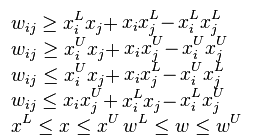
\includegraphics[scale=0.6]{env.png}
  \end{center}
\end{figure}

\paragraph{}\hl{For the $L_{\infty}$-norm we add constraints (29)--(30) to the barebones model:}

\begin{alignat}{3}
  &&& o_{k} \leq y && \quad \forall k \in \mathcal{B} \\
  &&& y \in \{d_{\min}, ..., d_{\max}\}
\end{alignat}

\hl{The $L_{\infty}$-norm kind of works right now, but still needs some refining.}


%\footnote{https://optimization.mccormick.northwestern.edu/index.php/McCormick\_envelopes}


%%%%%%%%%%%%%%%%%%%%%%%%%%%%%%%%%%%%%%%%%%%%%%%%%%%%%%%%%%%%%%%%%%%%%%%%%%%%%%%%%%%%%%%%%%%%%%%%%%%%
%%%%%%%%%%%%%%%%%%%%%%%%%%%%%%%%%%%%%%%%%%%%%%%%%%%%%%%%%%%%%%%%%%%%%%%%%%%%%%%%%%%%%%%%%%%%%%%%%%%%


% TODO: redo all this section
\section{IP Model B}
\label{sec:ip_model_b}

\paragraph{}Our second IP model (IP\textsubscript{B}) is based on the definition of an exponential-size collection of possible bin compositions as for the classical bin packing problem. Indeed, as for bin packing, the resulting formulation can be solved by column generation with either a set covering (SC) or set partitioning (SP) model. Let $\mathbb{S}$ be the collection of all subsets of items that can be packed into the same bin

\[
\mathbb{S} \coloneqq \left\{ S \subseteq \{1, \dots, n\} : \ell \leq \sum_{i \in S} w_{i} \leq u, \quad \forall i, j \in S:c_{ij} \neq \infty\right\}.
\]

We can observe that it may not be possible to \emph{only} construct maximal sets with regards to the bin capacity due to conflicts between items and the constraints enforcing them. There is a binary variable for each subset $S \in \mathbb{S}$ representing a combination of items, or \emph{pattern}, to be packed into the same bin

\begin{equation}
  x_{S}\coloneqq
  \begin{cases}
    1, & \mbox{if pattern $S$ is selected,} \\
    0, & \mbox{otherwise.}
  \end{cases}
\end{equation}

The sum of all pairwise costs for the items of a pattern and the deviation of the weight of that pattern from the mean bin load are represented by $\alpha$ and $\beta$, respectively. In regards to the balancing objective, using a fixed number of bins has two major advantages over using a variable number of bins. First, the values of $\alpha$ and $\beta$ need to be computed only once per pattern (when it is generated) and remain constant throughout the process. Second and more importantly, since $\beta$ is computed outside of the program, the norm according to which it is computed does not complexify the problem (i.e., the program remains linear even when balance is computed according to an $L_{2}$-norm).

While the solution of a SP model is always directly feasible, that of a SC model must be transformed in order to be feasible for our problem (i.e., we must remove all duplicate items from the bins). This has the unfortunate effect of potentially worsening the objective funtion. Example 1 illustrates the underlying issue of using a SC model to solve our problem.

\begin{example}
  Assume an instance of the problem with 2~bins and 4~items $A$, $B$, $C$, and $D$. The pairwise costs of $AB$, $BC$, $CD$, and $DA$ are~0, while the pairwise cost of $AC$ is~1 and that of $BD$ is~$-2$. We also have $\ell=2$ and $u=3$. The two most profitable maximal subsets are $ABD$ and $BCD$ which both have a value of~$-2$ and cover all the items. The initial solution of the SC model would be $(-2)+(-2)=-4$, which must be rendered feasible for our problem by removing $B$ from one bin and $D$ from the other. This modified solution would have a value of $(0)+(0)=0$, while the solution of a SP model would be to pack $AC$ and $BD$ in separate bins, for a value of $(1)+(-2)=-1$.
\end{example}

The master problem (MP) is thus based on a SP model.

\begin{alignat}{3}
  & \min \quad && \sum \limits_{S \in \mathbb{S}} \alpha_{S} x_{S} \\
  &\textrm{s.t.} \notag \\
  &&& \sum \limits_{S \in \mathbb{S}:i \in S} x_{S} = 1 && \quad \forall i \in \mathcal{I} \\
  &&& \sum \limits_{S \in \mathbb{S}} x_{S} = m \\
  &&& \sum \limits_{S \in \mathbb{S}} \beta_{S} x_{S} \geq d_{\min} && \\
  &&& \sum \limits_{S \in \mathbb{S}} \beta_{S} x_{S} \leq d_{\max} && \\
  &&& x_{S} \in \{0, 1\} && \quad \forall S \in \mathbb{S}
\end{alignat}

The MP minimizes the combined costs of all bins~(23), under the conditions that each item be packed into one and only one bin~(24), that a total of $m$ bins be used~(25), and that the cumulative deviation of a solution be within bounds~$d_{\min}$ and~$d_{\max}$~(26)-(27). In order to begin solving the problem, the column generation algorithm needs~$m$ columns making up an initial feasible solution of the problem and of the continuous relaxation obtained by replacing constraints (28) with $x_{S} \geq 0, \forall S \in \mathbb{S}$. These columns are generated by a compact CP model defined by (1)-(5), (7), (todo: and some symmetry breaking and simple search strategy), and

\begin{alignat}{3}
  & b_{i} \neq b_{j}, \quad && b_{i}, b_{j} \in \mathcal{B}, \quad \forall i, j \in \mathcal{I}:c_{ij}=\infty
\end{alignat}

\noindent which searches for the first feasible solution safisfying these constraints. The~$m$ columns found by this CP model make up the initial restricted master problem~(RMP). The dual of the MP is

\begin{alignat}{3}
  & \max \quad && \sum \limits_{i=1}^{n} y_{i} + m\zeta + d_{\min}\gamma + d_{\max}\delta \\
  &\textrm{s.t.} \notag \\
  &&& \sum \limits_{i \in S} y_{i} + \zeta + \beta_{S}(\gamma + \delta) \leq \alpha_{S} && \quad \forall S \in \mathbb{S} \\
  &&& y_{i} \text{ free} && \quad \forall i \in S \\
  &&& \zeta \text{ free} \\
  &&& \gamma \geq 0 \\
  &&& \delta \leq 0
\end{alignat}

\noindent which is all that is needed for the column generation algorithm to take over:

\begin{enumerate}
\item Solve the continuous relaxation of the RMP to get the dual values.
\item Solve the subproblem, or pricing problem (PP), to generate $S^{*} \subseteq \{1, \dots, n\}$ (the most promising new column). Let
\begin{equation}
  z_{i}\coloneqq
  \begin{cases}
    1, & \mbox{if item $i$ is packed into the new bin/pattern,} \\
    0, & \mbox{otherwise.}
  \end{cases}
\end{equation}
\hl{The pricing problem is now solved by a CP model and is about 10 times faster. Average results when solving an instance of 50 items: $L_1$-norm: time=5.7s, LB=-132, absolute gap=3; $L_2$-norm: time=2.6s, LB=-128, absolute gap=1.75. I still need to do the $L_{0}$- and $L_{\infty}$-norms.}

\begin{alignat}{3}
  & \max \quad && \sum \limits_{i=1}^{n} y_{i}^{*}z_{i} + \zeta^{*} + \beta(\gamma^{*}+\delta^{*}) - \sum \limits_{i=1}^{n-1} \sum \limits_{j=i+1}^{n} c_{ij} z_{i} z_{j} && \quad \text{if } \gamma^{*}+\delta^{*}<0 \label{eq:pp1} \\
  & \max \quad && \sum \limits_{i=1}^{n} y_{i}^{*}z_{i} + \zeta^{*} - \beta(\gamma^{*}+\delta^{*}) - \sum \limits_{i=1}^{n-1} \sum \limits_{j=i+1}^{n} c_{ij} z_{i} z_{j} && \quad \text{if } \gamma^{*}+\delta^{*}>0 \label{eq:pp2} \\
  &\textrm{s.t.} \notag \\
  &&& z_{i} + z_{j} \leq 1 && \quad \forall i,j \in \mathcal{I}:c_{ij}=\infty \label{eq:pp3} \\
  &&& \sum \limits_{i=1}^{n} w_{i} z_{i} \geq \ell && \label{eq:pp4} \\
  &&& \sum \limits_{i=1}^{n} w_{i} z_{i} \leq u && \label{eq:pp5} \\
  &&& \sum \limits_{i=1}^{n} w_{i} z_{i} - w/m \leq \beta && \label{eq:pp6} \\
  &&& \sum \limits_{i=1}^{n} w_{i} z_{i} - w/m \geq -\beta && \label{eq:pp7} \\
  &&& z_{i} \in \{0, 1\} && \quad \forall i \in \mathcal{I} \label{eq:pp8} 
\end{alignat}
The PP minimizes the value of a bin~(\ref{eq:pp1})/(\ref{eq:pp2}) under the conditions that no conflicting items be packed into it (\ref{eq:pp3}), and that its load be within bounds $\ell$ and $u$~(\ref{eq:pp4})-(\ref{eq:pp5}). Constraints~(\ref{eq:pp6})-(\ref{eq:pp7}) work in the same manner as constraints (15)-(16) and ensure that deviation $\beta$ is always positive.
\item Determine if $S^{*}$ should be added to the RMP. If the inequality $\sum_{k \in S^{*}} y_{k}^{*} + \zeta^{*} + \beta(\gamma^{*}+\delta^{*}) > \sum_{i \in S^{*}} \sum_{j \in S^{*}} c_{ij}$ (or $\sum_{k \in S^{*}} y_{k}^{*} + \zeta^{*} - \beta(\gamma^{*}+\delta^{*}) > \sum_{i \in S^{*}} \sum_{j \in S^{*}} c_{ij}$, alternatively) is true, compute $\alpha_{S^{*}}$ and $\beta_{S^{*}}$, and add column $S^{*}$ to the RMP before going back to step 1. Otherwise, the current solution of the continuous relaxation of the RMP is the lower bound of the initial problem.
\end{enumerate}

The optimal solution of the continuous relaxation of the RMP provides a lower bound to the problem. We subsequently enforce constraints (28) and solve the RMP with the columns which were previously generated by the algorithm in order to find an integral solution. We know such an integral solution exists since we started off with one with our initial columns. While this final integral solution offers no proof of optimality, it is most often relatively close to the lower bound.

Depending on the norm used to balance the bins and on the value of bound~$d_{\max}$, we can make arithmetic deductions to determine the optimal~$\ell$ and~$u$ bounds which should help prematurely prune nodes leading to infeasible solutions, without eliminating any feasible solution:

\hl{This will be updated to include the other norms.}
%As for the $L_{\infty}$-norm, all bins can always simultaneously account for the whole deviation~(38)-(39).

\begin{align}
  \ell & \geq \max\{0, \left\lceil w/m - d_{\max}/2 \right\rceil \} \label{eq:norms1} \\
  u & \leq \left\lfloor w/m + d_{\max}/2 \right\rfloor \label{eq:norms2} \\
  \ell & \geq \max\{0, \left\lceil w/m - \sqrt{d_{\max} \times (m-1)/m} \right\rceil \} \label{eq:norms3} \\
  u & \leq \left\lfloor w/m + \sqrt{d_{\max} \times (m-1)/m} \right\rfloor \label{eq:norms4}
\end{align}

%  \ell & \geq \max\{0, \left\lceil w/m - d_{\max} \right\rceil \} \\
%  u & \leq \left\lfloor w/m + d_{\max} \right\rfloor

For the $L_{1}$-norm, in the worst case a single bin can account for at most half of the deviation, since the cumulative weight in excess of the mean bin load will always be equal to the cumulative weight short of the mean bin load~(\ref{eq:norms1})-(\ref{eq:norms2}). For the $L_{2}$-norm we must also take the number of bins into account in order to tightly bound the most deviative bin~(\ref{eq:norms3})-(\ref{eq:norms4}). This offline optimization of bin load bounds makes a noticeable difference for both IP models, cutting the execution time by half on average. This optimization is of no use for the CP model, as the balancing constraint already ensures that bin loads be consistent with $d_{\max}$.

%\paragraph{}A branch-and-price algorithm is used to find an optimal or near-optimal (when opting for a relative gap tolerance cutoff) solution to the problem. The branch-and-price algorithm is essentially a branch-and-bound algorithm with column generation at each node. [NOTE: I'm working on a better branching heuristic which I'll mention here]


%%%%%%%%%%%%%%%%%%%%%%%%%%%%%%%%%%%%%%%%%%%%%%%%%%%%%%%%%%%%%%%%%%%%%%%%%%%%%%%%%%%%%%%%%%%%%%%%%%%%
%%%%%%%%%%%%%%%%%%%%%%%%%%%%%%%%%%%%%%%%%%%%%%%%%%%%%%%%%%%%%%%%%%%%%%%%%%%%%%%%%%%%%%%%%%%%%%%%%%%%

\section{\hl{MH Model}}
\label{sec:mh_model}

\hl{I propose to construct the metaheuristic model proposed by Lewis (tabu search) from scratch. It will be designed in line with our other models (i.e., the objective function only takes costs into account, and we build solutions with $d_{\min}$ and $d_{\max}$), take into account all the norms, construct a Pareto front, etc.}


%%%%%%%%%%%%%%%%%%%%%%%%%%%%%%%%%%%%%%%%%%%%%%%%%%%%%%%%%%%%%%%%%%%%%%%%%%%%%%%%%%%%%%%%%%%%%%%%%%%%
%%%%%%%%%%%%%%%%%%%%%%%%%%%%%%%%%%%%%%%%%%%%%%%%%%%%%%%%%%%%%%%%%%%%%%%%%%%%%%%%%%%%%%%%%%%%%%%%%%%%

\section{Benchmark Results}
\label{sec:benchmark_results}

\hl{I propose to remove the plain CP results and just keep the CP+LNS results, and mention textually what kind of improvement LNS offers.}

\paragraph{}Our testbed includes instances of 25 and 50 items, of weights chosen uniformly at random from 1 to 8 (in a similar fashion as Lewis~\cite{Lewis2013}). Costs and conflicts are introduced according to probability $p$ of a pairwise negative cost, probability $q$ of a pairwise positive cost, and probability $r$ of a conflict (i.e., $p+q+r \leq 1$, with the remainder being the probability that the pair incurs no cost). Costs range from~$-5$ to~5, and the number of bins has been chosen so that the mean load is closest to~10.

%The reason for this is that the branching heuristic basically packs the heaviest items near the top of the tree, with gradually lighter items packed on top of them until a feasible solution is reached at the bottom of the tree. Early backtracks are short and quickly improve this solution by essentially swapping around some of the lightest items near the bottom of the tree to pack them more profitably. A plateau is quickly reached, after which further improvements are few and far between. Fixing the maximum clique in separate bins often means packing some items of small weight near the top of the tree, which in turn won't be available near the bottom of the tree to improve the solution early on. Forcing an order on bin loads prevents some profitable pairs of items from being packed together early in the tree for the sake of symmetry breaking. The only profitable form of symmetry breaking involves fixing items whose weights are greater than half of the bin capacity, which does not interfere with the branching heuristic. These particularities are also the reason why limited discrepancy search (LDS) does not improve the quality of solutions.

The experiments were performed on dual core AMD~2.2~GHz processors with 8~GB of RAM running CentOS~7, and all models were constructed with IBM ILOG CPLEX Optimization Studio~v12.5. Pareto sets are constructed for the smallest integral ranges of deviations (i.e., min/max deviations of 0/1, 1/2, ..., 19/20). Time limits cover only one range of deviations, meaning that the results for one method, for one figure, involve solving 20 independent problems. This also means that construction of the Pareto sets is easily parallelizable and can be scaled to limited resources by modifying its resolution (e.g., if 4 instances can be solved in parallel, a lower-resolution Pareto set can be constructed with min/max deviations of 0/5, 6/10, 11/15, 16/20). Each data point shows the average results of 5 different cost matrices applied to the same set of items. All figures show the results for instances of 25 or 50 items with the deviations computed according to an $L_{1}$-norm. For Figs.~1-3 the cost probabilities are $p=0.25$, $q=0.25$, and $r=0.25$.

\begin{figure}[H]
  %\vspace{5cm}
  \begin{center}
    \caption[]{Instances of 25 items with a time limit of 600s.}
    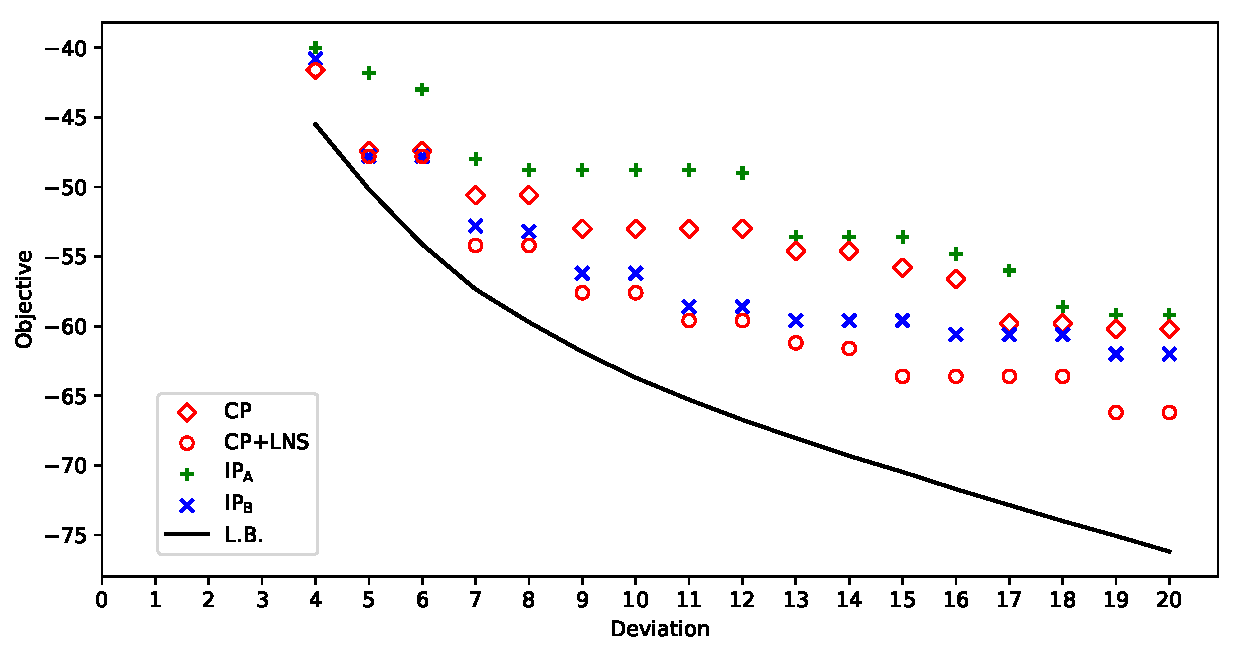
\includegraphics[scale=0.52]{new25-norm1-tl600.pdf}
  \end{center}
\end{figure}

\begin{figure}[H]
  %\vspace{5cm}
  \begin{center}
    \caption[]{Instances of 50 items with a time limit of 6s.}
    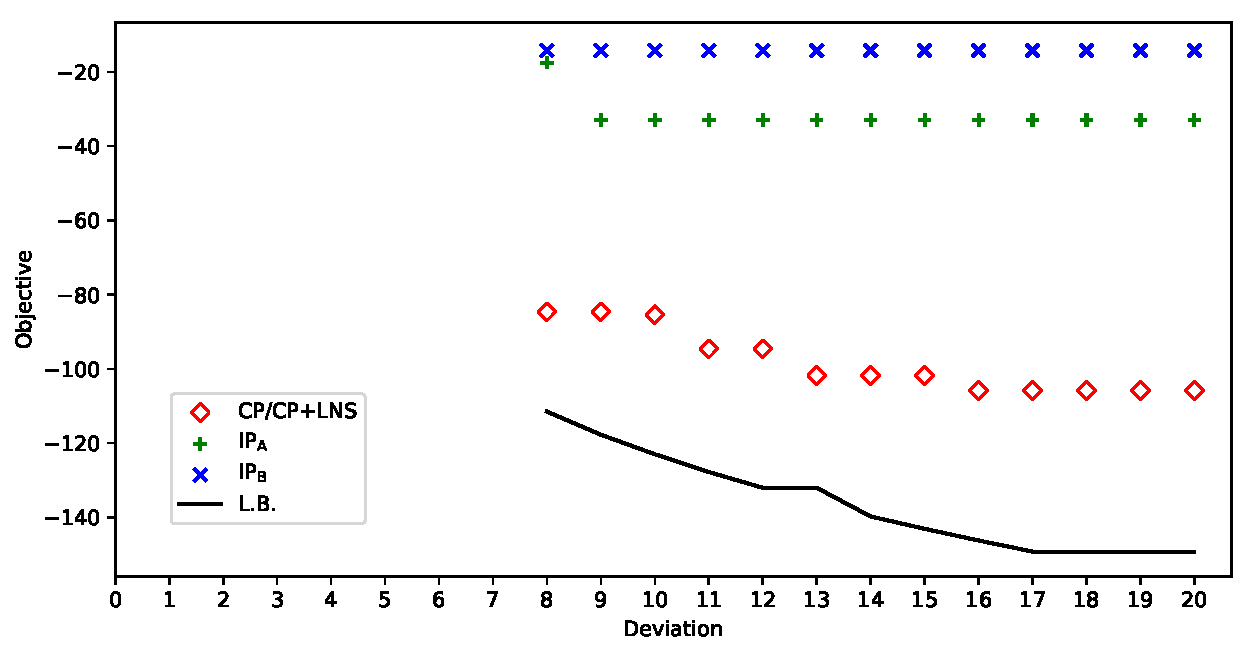
\includegraphics[scale=0.52]{new50-norm1-tl6.pdf}
  \end{center}
\end{figure}

\begin{figure}[H]
  %\vspace{5cm}
  \begin{center}
    \caption[]{Instances of 50 items with a time limit of 600s.}
    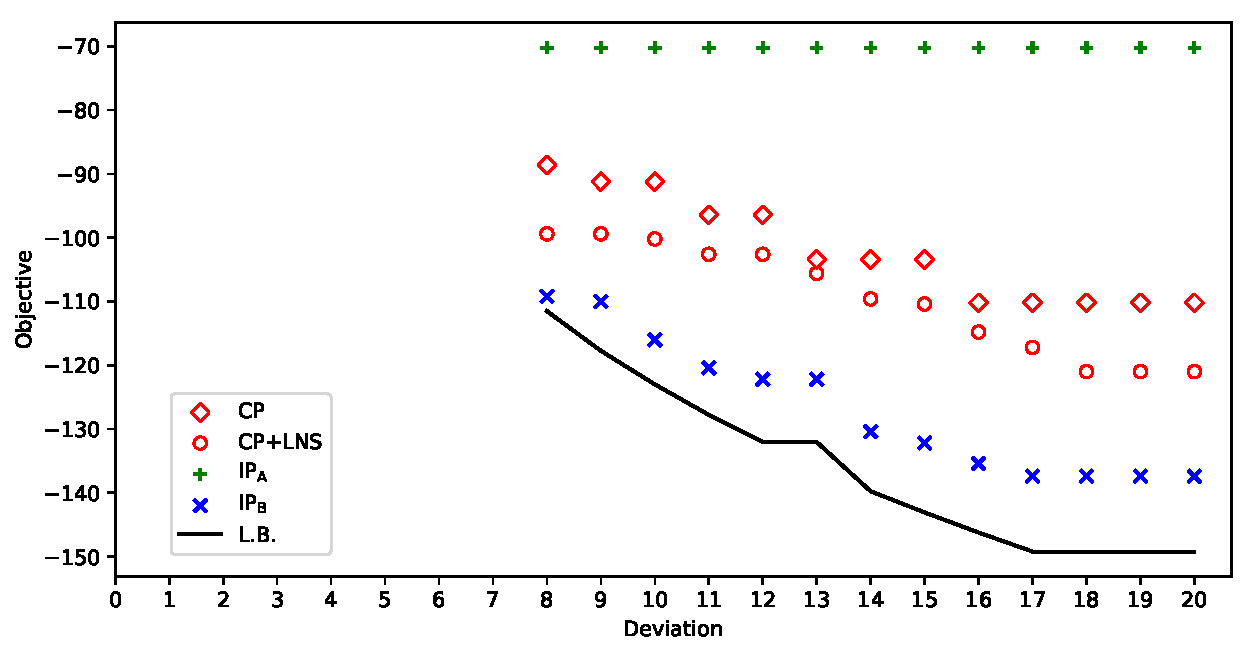
\includegraphics[scale=0.52]{new50-norm1-tl600.pdf}
  \end{center}
\end{figure}

We can observe in Fig. 2 that the CP model finds the best early solutions of all methods. However it quickly reaches a plateau from which it is hard to further improve (notice the similarity between the CP solutions of Fig. 2 with a time limit of 6s. and those of Fig. 3 with a time limit of 600s.). The introduction of LNS for the CP model always improves the solution quality. For the small instances of Fig. 1, the CP model with LNS does better than IP\textsubscript{B} since the latter only solves the relaxation of the RMP to optimality and tries to get the best integral solution from these limited columns, with no proof of optimality. IP\textsubscript{A} does particularly poorly compared with the other models. The results of IP\textsubscript{B} are usually off to a slow start, but given enough time this model does better than both previous ones. Similar to the CP model, this model reaches a plateau of its own before the 600s mark. Further improvements could be achieved via branch and price. Average computation times are shown in Table~1 (owing to details in the implementation of the models, the execution time may be slightly higher than the time limit in some cases).

%With 25 items, the solutions of IP\textsubscript{A} slowly converge towards those of the CP model, given enough time. This is not true with instances of 50 items, whose results for this model are far from those of the two others. The only advantage of IP\textsubscript{A} is that it can prove optimality or infeasibility for some 25-item instances, when the maximum deviation is low enough. 

\begin{table}[H]
  \centering
  \setlength{\tabcolsep}{8pt}
\caption{Average computation times for Figs. 1-3}
\begin{tabular}{lrrr}
  \cline{2-4}\noalign{\smallskip}
  & \multicolumn{1}{c}{25 items} & \multicolumn{2}{c}{50 items} \\
  \cline{2-4}\noalign{\smallskip}
& 600s. & 6s. & 600s. \\
\noalign{\smallskip}
\hline
\noalign{\smallskip}
CP    & 510.00 & 3.90 & 390.00 \\
CP+LNS & 508.49 & 3.90 & 379.02 \\
IP\textsubscript{A} & 589.06 & 6.96 & 602.04 \\
IP\textsubscript{B} & 8.35 & 8.32 & 178.46 \\
\hline
\end{tabular}
\end{table}

For the CP and IP\textsubscript{A} models, infeasibility or optimality can sometimes be proven when the maximum cumulative deviation is low enough. IP\textsubscript{B} does well especially when the time limit is high, although its solutions cannot be proven optimal without a branch-and-price scheme (but the CP model generating its initial columns can determine if an instance is infeasible). We have further tried solving instances with conflicts only ($p=0$, $q=0$, $r=0.25$) and every method could find a solution within the time limit. In Fig. 4 we show the results of instances without conflicts and only with costs ($p=0.25$, $q=0.25$, $r=0$).

\begin{figure}[H]
  \begin{center}
    \caption[]{Instances of 50 items with a time limit of 600s. (costs only)}
    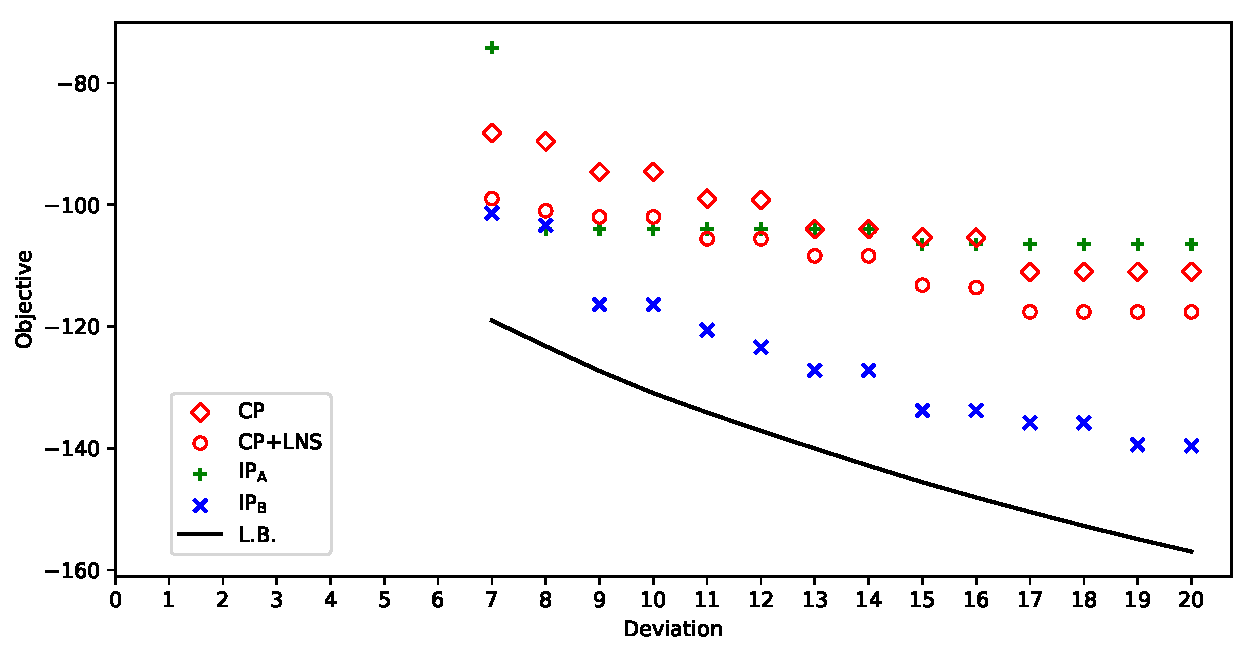
\includegraphics[scale=0.52]{cost50d-norm1-tl600.pdf}
  \end{center}
\end{figure}

\begin{table}[H]
  \centering
  \setlength{\tabcolsep}{8pt}
\caption{Average computation times}
\begin{tabular}{lrr}
  \cline{2-3}\noalign{\smallskip}
  & \multicolumn{2}{c}{50 items} \\
  \cline{2-3}\noalign{\smallskip}
& Conflicts only & Costs only \\
\noalign{\smallskip}
\hline
\noalign{\smallskip}
CP    & 0.03 & 420.00 \\
CP+LNS & 0.03 & 390.78 \\
IP\textsubscript{A} & 601.11 & 600.62 \\
IP\textsubscript{B} & 4.64 & 28.65 \\
\hline
\end{tabular}
\end{table}

It is interesting to notice that with only conflicts, the CP model very easily proves optimality for all instances in a fraction of a second, whereas both IP models are orders of magnitude behind it. The weakness of the CP model lies in the optimization of objective $f$, even with LNS. IP\textsubscript{A} appears to generally do better without conflicts, while the performance and results of IP\textsubscript{B} are largely unaffected by the parameters of the instances.

\paragraph{}A CP/IP\textsubscript{B} hybrid could be constructed: The CP part would generate the initial columns, those columns being the current CP solution once the model reaches its plateau; From there, the IP part would take over and improve this solution by bringing it to near-optimality. Experimentation would be necessary to see if such a model would be an improvement over current methods. We have not integrated the CP and IP\textsubscript{B} models into a hybrid in this paper, as our objective was to compare individual methods to each other. Furthermore, our simple approach to the generation of the Pareto sets for both IP models could be improved \cite{Boland2015}.

%%%%%%%%%%%%%%%%%%%%%%%%%%%%%%%%%%%%%%%%%%%%%%%%%%%%%%%%%%%%%%%%%%%%%%%%%%%%%%%%%%%%%%%%%%%%%%%%%%%%
%%%%%%%%%%%%%%%%%%%%%%%%%%%%%%%%%%%%%%%%%%%%%%%%%%%%%%%%%%%%%%%%%%%%%%%%%%%%%%%%%%%%%%%%%%%%%%%%%%%%


\section{\st{Practical Applications}}
\hl{I am thinking of removing this section and instead mentioning this application in another section. The objective of the metaheuristic model (as it is found on the website) is not similar to that of our models (cost+deviation in its objective, instead of only cost for our objectives, with the deviation as a constraint). Furthermore it is poorly coded (it does not take into account the negative costs, which it should) and it is not flexible (costs are either -1, 0, or 1, while we can test our own models with whatever range of costs we like). Finally, it only takes into account the $L_1$-norm. So I suggest removing this section, re-coding the metaheuristic model to our standards, and including it as another model alongside our CP and 2 IP models. This would thereby add a new contribution to this paper, by introducing new balancing schemes for a metaheuristic model.}

\paragraph{}\st{The metaheuristic approach developed by Lewis}~\cite{Lewis2013} \st{is used on the commercial website \texttt{www.weddingseatplanner.com} as a tool to generate seating plans. The problem is similar to ours which is described in Sect.~2 of this paper, with a few exceptions: Bin loads are unbounded, negative costs are always equal to $-1$ and positive costs are always equal to 1, and the deviation is computed according to an $L_{1}$-norm and directly added to the objective (i.e., the objective is to minimize $f$ plus the deviation). The objective functions of our models have been adapted for these tests.}

\st{One of the design goals of the website was to solve the problem \emph{quickly} since their clients could easily grow impatient after waiting just a few seconds in front of a seemingly unresponsive browser window. As such, their tool usually solves the problem in less than 5 seconds, a time limit which cannot be specified by the user. Because of this short time limit, we have bounded the maximum deviation of our models at 20 in order to find better results. For the CP model, since the balancing constraint and the branching heuristic are very effective, we have further decided to solve the instances two more times by bounding the maximum deviation at 10 and 5, respectively (since we are solving thrice as many problems, we have also divided the time limit by three). We will be considering only the best of those three solutions.}

\st{Due to an error in the website's implementation of the algorithm, all negative costs are considered to be conflicts. In order to provide a fair comparison, the instances we have generated for these tests do not include negative costs. The cost probabilities are thus $p=0$, $q=0.\bar{3}$, and $r=0.\bar{3}$ (which implies that the probability of a cost of 0 is also $0.\bar{3}$). Since the website always solves the instances in under 5 seconds, this is what we have chosen as our time limit. Tests have been run with 10, 20, 30, 40, and 50 items, and are again averaged for five cost matrices. The histograms shown in Fig.~5 represent the distance in score of a solution from the lower bound.}

\begin{figure}[H]
  \begin{center}
    \caption[]{All methods compared with a time limit of 5s.}
    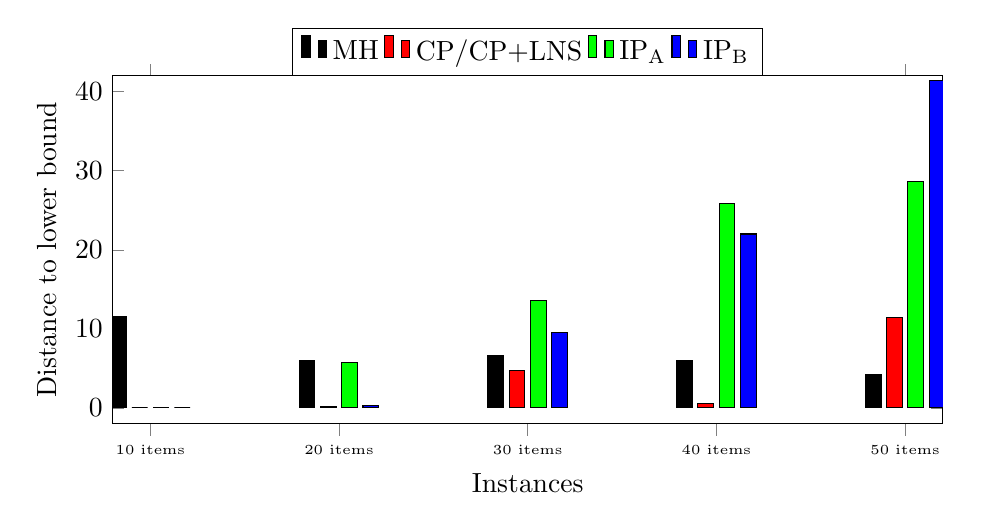
\begin{tikzpicture}
      \begin{axis}[
          ybar,
          width = \textwidth,
          height = 6cm,
          bar width = 2mm,
          enlargelimits=0.05,
          legend style={at={(0.5, 1)},
            anchor=south, legend columns=-1},
          ylabel={Distance to lower bound},
          xlabel={Instances},
          x tick label style={font=\tiny,text width=1cm,align=center},
          symbolic x coords={10 items,20 items,30 items,40 items,50 items},
          xtick=data,
          ymin=0, ymax=40,
        ]
        \addplot [fill=black] coordinates {(10 items,11.6) (20 items,6) (30 items,6.6) (40 items,6) (50 items,4.2)};
        \addplot [fill=red] coordinates   {(10 items,0) (20 items,0.2) (30 items,4.71) (40 items,0.6) (50 items,11.4)};
        \addplot [fill=green] coordinates {(10 items,0) (20 items,5.8) (30 items,13.6) (40 items,25.9) (50 items,28.6)};
        \addplot [fill=blue] coordinates  {(10 items,0) (20 items,0.3) (30 items,9.5) (40 items,22) (50 items,41.4)};
        \legend{MH, CP/CP+LNS, IP\textsubscript{A}, IP\textsubscript{B}}
      \end{axis}
    \end{tikzpicture}
  \end{center}
\end{figure}

\st{When solving small instances, exact methods have a distinct advantage over metaheuristics, often proving optimality. Both IP models scale poorly with an increasing number of items as they usually require some time to find decent solutions. While it can find the best solutions given enough time, }IP\textsubscript{B} \st{does particularly badly with a short time limit as the quality of its solutions improves relatively slowly. The metaheuristic model scales very well, with its solution quality being constant with a varying number of items. The CP model does well all-around, proving optimality for small instances as well as having good solutions for all instances.}

%\paragraph{}The WSP is more of a toy problem, and one should take note that the very nature of WSP implies that a machine is unqualified to properly solve it. Assigning guests to tables for a wedding is part of the tradition for the engaged couple who are planning the most important day of their lives. They are emotionally invested in this task. A machine with perfect information achieving a proven optimal solution will still fall short of the \emph{best} assignment since the emotional factor associated with the problem cannot be integrated into the model. However, the WSP could be a good test case for similar problems of a different nature, such as assigning business associates and competitors around tables in a big meeting. (GP NOTE: We should mention this already in the introduction as motivation for our work [that the WSP is a test case for other problems])


%%%%%%%%%%%%%%%%%%%%%%%%%%%%%%%%%%%%%%%%%%%%%%%%%%%%%%%%%%%%%%%%%%%%%%%%%%%%%%%%%%%%%%%%%%%%%%%%%%%%
%%%%%%%%%%%%%%%%%%%%%%%%%%%%%%%%%%%%%%%%%%%%%%%%%%%%%%%%%%%%%%%%%%%%%%%%%%%%%%%%%%%%%%%%%%%%%%%%%%%%


\section{Conclusion}

\paragraph{}In this paper we have compared how various methods can be used to solve multi-objective constrained bin packing problems with an aspect of load balancing. A metaheuristic model can find good solutions in a short time and scales well to an increasing number of items but will most likely not find optimal solutions. A CP model can also find good solutions quickly, but for large instances it will not reach the best solutions in reasonable time even with the help of LNS. A natural IP model is probably not the best choice, as it scales poorly while its strenghts can also be found in other models. An IP model using column generation does very well given enough time but is not a good contender to solving instances quickly. It would be interesting to see if a CP/IP hybrid using column generation and branch and price could prove optimality in reasonable time for larger instances of the problem.

\section*{Acknowledgements}

\paragraph{}Financial support for this research was provided by NSERC Discovery Grant 218028/2017 and CERC, École Polytechnique de Montréal.

\bibliography{references}{}
\bibliographystyle{splncs}


\end{document}



%%%%%%%%%%%%%%%%%%%%%%%%%%%%%%%%%%%%%%%%%%%%%%%%%%%%%%%%%%%%%%%%%%%%%%%%%%%%%%%%%%%%%%%%%%%%%%%%%%%%
%%%%%%%%%%%%%%%%%%%%%%%%%%%%%%%%%%%%%%%%%%%%%%%%%%%%%%%%%%%%%%%%%%%%%%%%%%%%%%%%%%%%%%%%%%%%%%%%%%%%







\newpage
\paragraph{}Toutes les instances ont 50 items avec une limite de temps de 600s. Entre parenthèses dans la légende est le temps d'exécution moyen.

\begin{figure}[H]
  \begin{center}
    \caption[]{50 items, 600s, 0.2 conflits}
    \includegraphics[scale=0.5]{../results/lb002.pdf}
  \end{center}
\end{figure}

\paragraph{}Quand il n'y a que des conflits, l'heuristique originale réussit particulièrement bien (suspicieusement trop bien?), contrairement à la nouvelle.

\begin{figure}[H]
  \begin{center}
    \caption[]{50 items, 600s, 0.2 "rather apart"}
    \includegraphics[scale=0.5]{../results/lb020.pdf}
  \end{center}
\end{figure}

\paragraph{}Quand il n'y a que des coûts positifs c'est la nouvelle heuristique qui fonctionne mieux. De plus, l'heuristique originale ne trouve pas certaines solutions (étrange? des solutions avec une valeur positive devraient être faciles à trouver. Il doit y avoir un problème...?)

\begin{figure}[H]
  \begin{center}
    \caption[]{50 items, 600s, 0.2 "rather together"}
    \includegraphics[scale=0.5]{../results/lb200.pdf}
  \end{center}
\end{figure}

\paragraph{}Quand il n'y a que des coûts négatifs l'heuristique originale fonctionne mieux.

\begin{figure}[H]
  \begin{center}
    \caption[]{50 items, 600s, 0.1 partout}
    \includegraphics[scale=0.5]{../results/lb111.pdf}
  \end{center}
\end{figure}

\paragraph{}Avec un peu de tout l'heuristique originale fonctionne mieux.

\paragraph{}Je crois qu'il y a possiblement un problème avec la façon dont l'heuristique originale gère les coûts positifs. Je vais regarder ça.

\newpage










%23 nov: CP: symmetry breaking of bin loads is harmful to the branching heuristic. For example, in order to put the most profitable item with an item which was fixed near the top of the tree, if it would mean that that bin's load would not respect the symmetry-breaking constraint, then we would have to backtrack up to the top if we were to put that item there. So we end up putting a suboptimal item with him instead. So, the only type of SB which works well is fixing items in bins at the start.

weakness: when the weights are all similar, this creates a weakness for the colgen approach, as a similar score can be reached in many different ways

%sb: decreasing bin values (so fill the bins as best as possible first). so no item fixing in the beginning

%the cp model is outperformed by the ipb, however it can find a better solution after just a few seconds, which can possibly be useful for certain applications

%ipa could handle l2 norm with mccormick inequalities

%17 nov: LDS does not work all the time, sometimes it does not work very well with the branching heuristic.

%Presenting the results: Have a table with the LP solution, IP solution (with only the columns of the LP without BaP), IP solution with BaP, computation time, number of columns. For CP: number of fails, etc.

%nov14: for CPA, nondecreasing table occupancy for symmetry brreaking is VERY bad for some reason. Also, cliques are good but for very low deviations (ex. deviation bounds of 0-1 or 1-2 or something) they are too long to compute. We can either break symmetry by fixing groups of too big size (size > ubound/2), or find cliques with a heuristic. SO, modify CP part about bron-kerbosch and say that cliques should be computed heuristically rather than B-K since it is more reliable when the deviation is too small

%nov14: What is the impact of the choice of \ell and u on the performance? [from draft1 GP correction] -> we will not explore this, we are using autobounds only

%nov 10: For IP model A, for pareto, the following observation: bounding the deviation with a lower AND upper bound at the same time takes a bit more time to solve than just bounding it with a maximum deviation (usually). So to compute for the pareto set, just bound max deviation

%[6nov2017] computation time for the pareto set is computed for the whole set (i.e., for a 20 minute cutoff with deviation going from 0 to 20, set the time limit for each deviation to 1 minute). Take note of the increased time needed to solve instances with a higher deviation bound

[6nov2017] If there are all different integer costs (i.e., all costs are for e.g. -10 to 10 instead of -1 to 1) then there will be much less symmetry and it should be easier to branch and price

%How were the p/q combinations chosen? [26oct2017] : I say we have 1/3 DA, 1/3 some kind of cost, and 1/3 no cost. Why? Because there are too many variations to try (number of groups, deviation type, range of item weights, range of item costs, etc.) that we are just trying on something "general", and there is not enough room in the paper to explore the extremes of every parameter and how it compares to the others. The models may not be very efficient for some types of instances (e.g., the CP model will probably do poorly on an instance with 90\% DA since just computing the cliques with the B-K algorithm could be intractable in itself)

%nov 10: IPA cannot handle an L2-norm! There seems to be no way around this. So IPB and CP have this advantage over IPA where they can use an L2 norm. So in this way they are more flexible.

%add a note that the CP solution is not the best, but a very good solution is found very fast, and this is what the advantage is [18oct2017]

%Explain that p and q were changed (p+q can only amount to 1). Or maybe: p=DA, q=RT/RA, r=no cost. So p+q+r=1

%nov 21: explain that CPA often proves optimality when the maxdev bound is still low, but that CP gets better results overall

mention that the branch and price algorithm doesn't work as well when the weights are too similar, e.g., if it is all 0, -1, and 1. That is because when we branch on a pattern, the colgen algorithm can often find a slightly different way of expressing a solution by using a similar pattern which will again be fractional. But with costs which are more variable, this is more easily fixed.

% THE relative gap is set at 1%

% preciser les details du WSP (que c'est +1 -1 les relations, et le balancement L1)

% also: show results of the first IP model (the one of lewis) for small instances

%Groups of size 1-4 are indentified as \emph{small groups} and groups of size 5-8 as \emph{large groups}. Three \emph{groups layouts} of varying group distributions were generated: the \emph{random groups layout} which has its group sizes chosen uniformly at random, the \emph{small groups layout} with twice as many small groups as large groups, and the \emph{large groups layout} with twice as many large groups as small groups.

%Relations matrices of 10 different types were generated according to two criteria: probability $p$ that a pair of groups should be \emph{definitely apart}, and probability $q$ that a pair of groups should be \emph{rather together}, \emph{rather apart}, or \emph{indifferent} (chosen randomly). Each groups layout has been combined with each relations matrix to form the 30 test instances.

%21 nov: auto-bounds on bin loads always help for IPA, cutting the execution time by up to half in many cases.
%21 nov.: auto-bounds seems to help for the CP model also. GP says it shouldn't normally help, so maybe do a bit more tests and then speak to him about it.

\begin{figure}[H]
  \vspace{0 cm}
  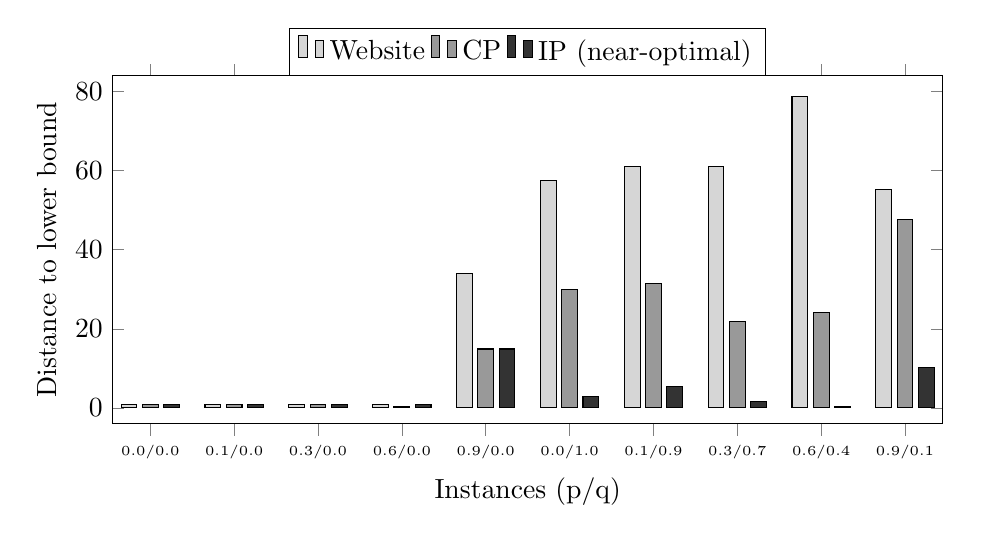
\begin{tikzpicture}
  % SMALL
\begin{axis}[
    ybar,
    width = \textwidth,
    height = 6cm,
    bar width = 2mm,
    enlargelimits=0.05,
    legend style={at={(0.5, 1)},
      anchor=south, legend columns=-1},
    ylabel={Distance to lower bound},
    xlabel={Instances (p/q)},
    x tick label style={font=\tiny,text width=1cm,align=center},
    symbolic x coords={0.0/0.0,0.1/0.0,0.3/0.0,0.6/0.0,0.9/0.0, 0.0/1.0,0.1/0.9,0.3/0.7,0.6/0.4,0.9/0.1},
    xtick=data,
    ymin=0, ymax=80,
    ]
\addplot [fill=gray!32] coordinates {(0.0/0.0,0.88) (0.1/0.0,0.88) (0.3/0.0,0.88) (0.6/0.0,0.88) (0.9/0.0,34) (0.0/1.0,57.61) (0.1/0.9,61.03) (0.3/0.7,61.07) (0.6/0.4,78.81) (0.9/0.1,55.24)};
\addplot [fill=gray!80] coordinates {(0.0/0.0,0.88) (0.1/0.0,0.88) (0.3/0.0,0.88) (0.6/0.0,0.46) (0.9/0.0,14.9) (0.0/1.0,30.03) (0.1/0.9,31.55) (0.3/0.7,21.8) (0.6/0.4,24.13) (0.9/0.1,47.73)};
\addplot [fill=gray!160] coordinates {(0.0/0.0,0.88) (0.1/0.0,0.88) (0.3/0.0,0.88) (0.6/0.0,0.88) (0.9/0.0,14.9) (0.0/1.0,2.82) (0.1/0.9,5.34) (0.3/0.7,1.59) (0.6/0.4,0.23) (0.9/0.1,10.25)};
\legend{Website, CP, IP (near-optimal)}
\end{axis}
\end{tikzpicture}
\caption[ ]{Results of the methods on instances of the \emph{small groups layout} type.}
\end{figure}

\begin{figure}[H]
  \vspace{0 cm}
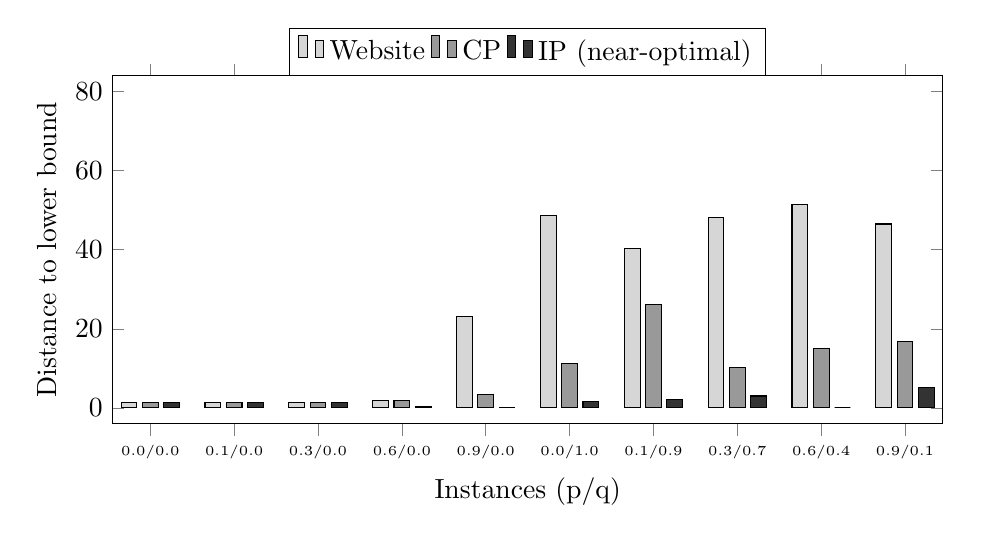
\begin{tikzpicture}
  % RANDOM
\begin{axis}[
    ybar,
    width = \textwidth,
    height = 6cm,
    bar width = 2mm,
    enlargelimits=0.05,
    legend style={at={(0.5, 1)},
      anchor=south, legend columns=-1},
    ylabel={Distance to lower bound},
    xlabel={Instances (p/q)},
    x tick label style={font=\tiny,text width=1cm,align=center},
    symbolic x coords={0.0/0.0,0.1/0.0,0.3/0.0,0.6/0.0,0.9/0.0, 0.0/1.0,0.1/0.9,0.3/0.7,0.6/0.4,0.9/0.1},
    xtick=data,
    ymin=0, ymax=80,
    ]
\addplot [fill=gray!32] coordinates {(0.0/0.0,1.48) (0.1/0.0,1.48) (0.3/0.0,1.48) (0.6/0.0,1.98) (0.9/0.0,23.16) (0.0/1.0,48.63) (0.1/0.9,40.39) (0.3/0.7,48.11) (0.6/0.4,51.36) (0.9/0.1,46.51)};
\addplot [fill=gray!80] coordinates {(0.0/0.0,1.48) (0.1/0.0,1.48) (0.3/0.0,1.48) (0.6/0.0,1.98) (0.9/0.0,3.44) (0.0/1.0,11.26) (0.1/0.9,26.21) (0.3/0.7,10.29) (0.6/0.4,15) (0.9/0.1,16.89)};
\addplot [fill=gray!160] coordinates {(0.0/0.0,1.48) (0.1/0.0,1.48) (0.3/0.0,1.48) (0.6/0.0,0.25) (0.9/0.0,0.13) (0.0/1.0,1.53) (0.1/0.9,2.21) (0.3/0.7,3.02) (0.6/0.4,0) (0.9/0.1,5.24)};
\legend{Website, CP, IP (near-optimal)}
\end{axis}
\end{tikzpicture}
\caption[ ]{Results of the methods on instances of the \emph{random groups layout} type.}
\end{figure}

\begin{figure}[H]
  \vspace{0 cm}
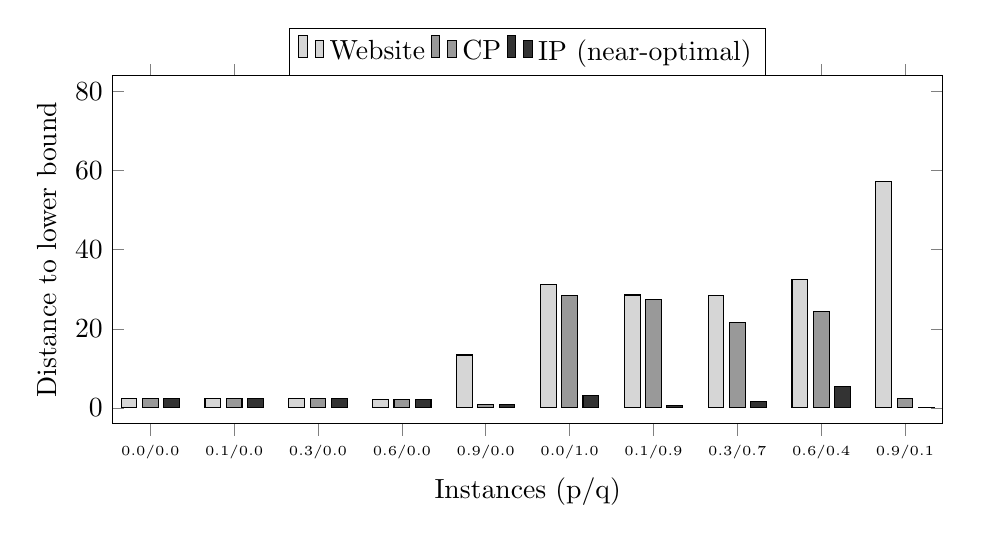
\begin{tikzpicture}
  % LARGE
\begin{axis}[
    ybar,
    width = \textwidth,
    height = 6cm,
    bar width = 2mm,
    enlargelimits=0.05,
    legend style={at={(0.5, 1)},
      anchor=south, legend columns=-1},
    ylabel={Distance to lower bound},
    xlabel={Instances (p/q)},
    x tick label style={font=\tiny,text width=1cm,align=center},
    symbolic x coords={0.0/0.0,0.1/0.0,0.3/0.0,0.6/0.0,0.9/0.0, 0.0/1.0,0.1/0.9,0.3/0.7,0.6/0.4,0.9/0.1},
    xtick=data,
    ymin=0, ymax=80,
    ]
\addplot [fill=gray!32] coordinates {(0.0/0.0,2.27) (0.1/0.0,2.27) (0.3/0.0,2.27) (0.6/0.0,2.19) (0.9/0.0,13.39) (0.0/1.0,31.27) (0.1/0.9,28.56) (0.3/0.7,28.48) (0.6/0.4,32.45) (0.9/0.1,57.19)};
\addplot [fill=gray!80] coordinates {(0.0/0.0,2.27) (0.1/0.0,2.27) (0.3/0.0,2.27) (0.6/0.0,2.19) (0.9/0.0,0.83) (0.0/1.0,28.35) (0.1/0.9,27.48) (0.3/0.7,21.55) (0.6/0.4,24.37) (0.9/0.1,2.33)};
\addplot [fill=gray!160] coordinates {(0.0/0.0,2.27) (0.1/0.0,2.35) (0.3/0.0,2.27) (0.6/0.0,2.19) (0.9/0.0,0.83) (0.0/1.0,3.2) (0.1/0.9,0.71) (0.3/0.7,1.55) (0.6/0.4,5.45) (0.9/0.1,0.12)};
\legend{Website, CP, IP (near-optimal)}
\end{axis}
\end{tikzpicture}
\caption[ ]{Results of the methods on instances of the \emph{large groups layout} type.}
\end{figure}

\begin{figure}[H]
  \vspace{0 cm}
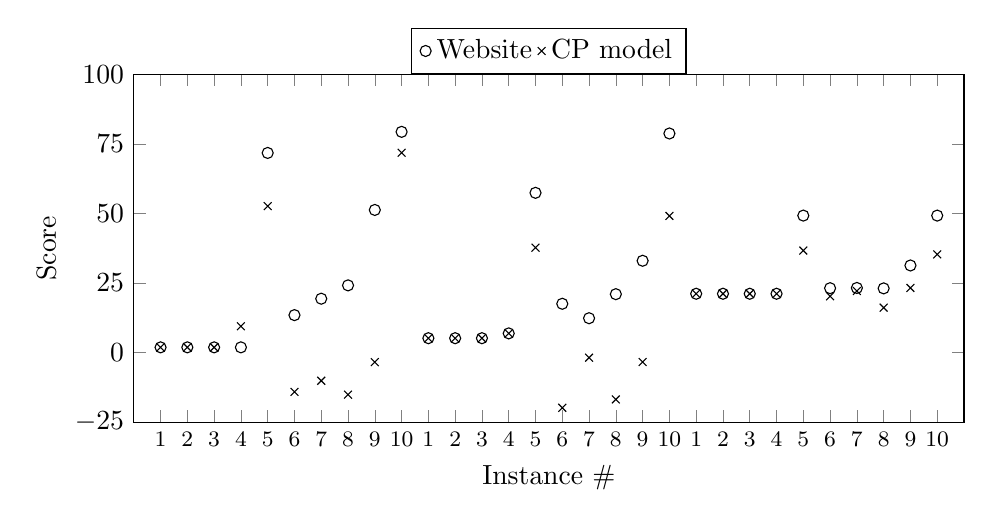
\begin{tikzpicture}
  \begin{axis}[%
      width = \textwidth,
      height = 6cm,
      %ymin=-50, ymax=100,
      %ytick={-50, -25, ..., 100},
      ymin=-25, ymax=100,
      ytick={-25, 0, ..., 100},
      xtick=data,
      legend style={at={(0.5, 1)},
        anchor=south, legend columns=-1},
	scatter/classes={%
		%a={mark=square*,blue},%
		%b={mark=triangle*,red},%
		%c={mark=o,draw=black},
                %d={mark=square*,green},
        	w={mark=o,black},%
		c={mark=x,black}},%,
		%i={mark=o,draw=black},
                %l={mark=square*,green}},
        ylabel={Score},
        xlabel={Instance \#},
        xmin=0, xmax=31,
        xticklabels={\footnotesize $1$, \footnotesize$2$, \footnotesize$3$, \footnotesize$4$, \footnotesize$5$, \footnotesize$6$, \footnotesize$7$, \footnotesize$8$, \footnotesize$9$, \footnotesize$10$, \footnotesize $1$, \footnotesize$2$, \footnotesize$3$, \footnotesize$4$, \footnotesize$5$, \footnotesize$6$, \footnotesize$7$, \footnotesize$8$, \footnotesize$9$, \footnotesize$10$, \footnotesize $1$, \footnotesize$2$, \footnotesize$3$, \footnotesize$4$, \footnotesize$5$, \footnotesize$6$, \footnotesize$7$, \footnotesize$8$, \footnotesize$9$, \footnotesize$10$}]
        %xticklabels={\footnotesize $s_{1}$, \footnotesize$s_{2}$, \footnotesize$s_{3}$, \footnotesize$s_{4}$, \footnotesize$s_{5}$, \footnotesize$s_{6}$, \footnotesize$s_{7}$, \footnotesize$s_{8}$, \footnotesize$s_{9}$, \footnotesize$s_{10}$, \footnotesize$r_{1}$, \footnotesize$r_{2}$, \footnotesize$r_{3}$, \footnotesize$r_{4}$, \footnotesize$r_{5}$, \footnotesize$r_{6}$, \footnotesize$r_{7}$, \footnotesize$r_{8}$, \footnotesize$r_{9}$, \footnotesize$r_{10}$, \footnotesize$l_{1}$, \footnotesize$l_{2}$, \footnotesize$l_{3}$, \footnotesize$l_{4}$, \footnotesize$l_{5}$, \footnotesize$l_{6}$, \footnotesize$l_{7}$, \footnotesize$l_{8}$, \footnotesize$l_{9}$, \footnotesize$l_{10}$}]
	\addplot[scatter,only marks,%
		scatter src=explicit symbolic]%
	table[meta=label] {
x     y      label
1 1.89 w
1 1.89 c
%1 1.89 i
%1 1.01 l
2 1.89 w
2 1.89 c
%2 1.89 i
%2 1.01 l
3 1.89 w
3 1.89 c
%3 1.89 i
%3 1.01 l
4 1.89 w
4 9.47 c
%4 1.89 i
%4 1.01 l
5 71.74 w
5 52.64 c
%5 52.64 i
%5 37.74 l
6 13.47 w
6 -14.11 c
%6 -41.32 i
%6 -44.14 l
7 19.37 w
7 -10.11 c
%7 -36.32 i
%7 -41.66 l
8 24.16 w
8 -15.11 c
%8 -35.32 i
%8 -36.91 l
9 51.26 w
9 -3.42 c
%9 -27.32 i
%9 -27.55 l
10 79.32 w
10 71.81 c
%10 34.33 i
%10 24.04 l
11 5.18 w
11 5.18 c
%11 5.18 i
%11 3.70 l
12 5.18 w
12 5.18 c
%12 5.18 i
%12 3.70 l
13 5.18 w
13 5.18 c
%13 5.18 i
%13 3.70 l
14 6.91 w
14 6.91 c
%14 5.18 i
%14 4.93 l
15 57.41 w
15 37.69 c
%15 34.38 i
%15 34.25 l
16 17.55 w
16 -19.82 c
%16 -29.55 i
%16 -31.08 l
17 12.36 w
17 -1.82 c
%17 -25.82 i
%17 -28.03 l
18 21 w
18 -16.82 c
%18 -24.09 i
%18 -27.11 l
19 33 w
19 -3.36 c
%19 -18.36 i
%19 -18.36 l
20 78.73 w
20 49.11 c
%20 37.46 i
%20 32.22 l
21 21.15 w
21 21.15 c
%21 21.15 i
%21 18.88 l
22 21.15 w
22 21.15 c
%22 21.15 i
%22 18.88 l
23 21.15 w
23 21.15 c
%23 21.15 i
%23 18.88 l
24 21.15 w
24 21.15 c
%24 21.15 i
%24 18.88 l
25 49.23 w
25 36.67 c
%25 36.67 i
%25 35.84 l
26 23.15 w
26 20.23 c
%26 -4.92 i
%26 -8.12 l
27 23.23 w
27 22.15 c
%27 -4.62 i
%27 -5.33 l
28 23.08 w
28 16.15 c
%28 -3.85 i
%28 -5.4 l
29 31.31 w
29 23.23 c
%29 4.31 i
%29 -1.14 l
30 49.23 w
30 35.29 c
%30 33.08 i
%30 32.96 l 
	};
        \legend{Website, CP model}
	\end{axis}
\end{tikzpicture}
\caption[ ]{Comparison between the website and the CP model.}
\end{figure}

\paragraph{}As long as there are only \emph{definitely apart} constraints, and not too many of them, both the metaheuristics approach and the CP model tend to find solutions very close to the optimum. The introduction of soft constraints, namely \emph{rather together} and \emph{rather apart}, is what sets apart the two methods. The metaheuristics approach does poorly with the addition of soft constraints, while the CP model almost always achieves better results with them than without.

\paragraph{}Solutions of instances with many small groups tend to have a lower optimum, which can be explained by two factors. Firstly, the cumulative deviation should be better because it is naturally easier to evenly fill bins with small items than with larger ones.

REPHRASE THIS: Secondly, the relational score should also be better since while the number of groups sitting at a table increases linearly, the table score could increase at a higher than linear rate (for example, while the second group being seated might increase the table score by only 1, the $n^{\text{th}}$ group being seated could potentially increase the score by $n-1$). Instances of the \emph{large groups layout} type do poorly when compared to other groups layouts. The reasons for this are similar to, albeit the reverse of, those previously mentioned. To begin with, it is harder to evenly split large items into bins of a limited capacity, since there is not a lot of wiggle room to play with. In addition, since we can fit on average fewer groups per table, and since the score of a table increases at a rate superior to that of the groups that can fit on it, a lower groups-per-table ratio is doomed to fetch a lower score.

\paragraph{}Some summary tests were achieved for smaller instances. For instances of 15 groups, the CP model proved optimality in under a second while the metaheuristics approach did even worse than what it could achieve on larger instances. (talk about IP, colgen, etc.) The metaheuristics approach probably lacks a proper strategy to deal with small instances.


%%%%%%%%%%%%%%%%%%%%%%%%%%%%%%%%%%%%%%%%%%%%%%%%%%%%%%%%%%%%%%%%%%%%%%%%%%%%%%%%%%%%%%%%%%%%%%%%%%%%
%%%%%%%%%%%%%%%%%%%%%%%%%%%%%%%%%%%%%%%%%%%%%%%%%%%%%%%%%%%%%%%%%%%%%%%%%%%%%%%%%%%%%%%%%%%%%%%%%%%%




%%%%%%%%%%%%%%%%%%%%%%%%%%%%%%%%%%%%%%%%%%%%%%%%%%%%%%%%%%%%%%%%%%%%%%%%%%%%%%%%%%%%%%%%%%%%%%%%%%%%
%%%%%%%%%%%%%%%%%%%%%%%%%%%%%%%%%%%%%%%%%%%%%%%%%%%%%%%%%%%%%%%%%%%%%%%%%%%%%%%%%%%%%%%%%%%%%%%%%%%%


\subsection*{Computing Problem-Specific Feasible Deviations}

\paragraph{}There exists only a small, finite set of feasible deviations for any given problem, which can be easily computed prior to solving the problem itself. All that is required is that the mean bin load be constant (i.e., the combined weight of the items as well as the number of bins must be fixed) and that the weights be integral. The intuition is that balancing loads amongst bins is a zero-sum game of sorts: the items taken out of a bin must necessarily packed into the others. There also exists a unique minimum feasible deviation for a problem, that is, when all bin loads are equal to the lower or upper integral part of the mean bin load. Since weight can be moved between bins only in integer amounts, and since there exists only one minimum feasible deviation to begin with, then any increase in deviation from the minimum is bound to be integral. The minimum feasible deviation of a problem can be computed with (31) for the L\textsubscript{1}-norm and with (32) for the L\textsubscript{2}-norm:

\begin{align}
  &2 \times m \times \left( \left\lceil m/w \right\rceil - m/w \right) \times \left( m/w - \left \lfloor m/w \right \rfloor \right) \\
  &m \times \left( \left\lceil m/w \right\rceil - m/w \right) \times \left( m/w - \left \lfloor m/w \right \rfloor \right)
\end{align}

\paragraph{}Starting at the minimum feasible deviation, for both norms, deviation can only increase in increments of 2. For the L\textsubscript{1}-norm this is obvious: moving a load of $l$ from one bin to another can result in one of three cases:

\begin{enumerate}
\item Both bins increase by $l$ in deviation, thus increasing the global deviation by $2 \times l$, or
\item Both bins decrease by $l$ in deviation, thus decreasing the global deviation by $2 \times l$, or
\item One bin increases by $l$ and the other decreases by $l$ in deviation, leaving the global deviation unchanged.
\end{enumerate}

\paragraph{}For the L\textsubscript{2}-norm it is not as obvious, and we have to examine all possible cases. For a general problem, let $f$ be the fractional part of the mean bin load such that $\left \lfloor w/m \right \rfloor + f = w/m$. The non-squared deviation of a bin will be fractional, and of one of two types: $(x+f)$ or $(x-f)$, with $x$ being some integer (e.g. for a mean of 10.3 the possible non-squared bin deviations are 0.3, 0.7, 1.3, 1.7...). Suppose we have two bins, $A$ and $B$, with $a$ and $b$ being, respectively, the integral part of their non-squared deviation. Bin $A$ can have a non-squared deviation of the type $(a+f)$ or $\left( a+(1-f) \right)$, and bin $B$ of the type $(b+f)$ or $\left( b+(1-f) \right)$. Let $c$ be the non-squared deviation modifier incurred by the bins when some load is traded from one to the other ($c$ is integral since all weights are integral). There are two cases to examine:

\begin{enumerate}
\item Both bins are of the same type: $(a+f)$ and $(b+f)$ with their loads below the mean, or $\left( a+(1-f) \right)$ and $\left( b+(1-f) \right)$ with their loads above the mean. In both cases, the bin loads are on the same side of the mean.
  \begin{enumerate}
  \item The deviations cannot both decrease.
  \item If $c<(b+f) \leq (a+f)$ or $c<(b+(1-f)) \leq (a+(1-f))$, both bin loads will remain on the same side of the mean. The difference in squared deviation will be $\left( (a+f+c)^{2} + (b+f-c)^{2} \right) - \left( (a+f)^{2} + (b+f)^{2} \right) = 2c^{2}+2ac-2bc$ in one case, and $\left( (a+(1-f)+c)^{2} + (b+(1-f)-c)^{2} \right) - \left( (a+(1-f))^{2} + (b+(1-f))^{2} \right) = 2c^{2}+2ac-2bc$ in the other case, with both of these differences being integral and multiples of 2.    
  \item If $c>(b+f)$ and $(b+f) \leq (a+f)$, or $c>(b+(1-f))$ and $(b+(1-f)) \leq (a+(1-f))$, the load of bin $B$ will shift to the other side of the mean. The difference in squared deviation will be $\left( (a+f+c)^{2} + (b+f+c-2(b+f))^{2} \right) - \left( (a+f)^{2} + (b+f)^{2} \right) = 2c^{2}+2ac-2bc$ in one case, and $\left( (a+(1-f)+c)^{2} + (b+(1-f)+c-2(b+(1-f)))^{2} \right) - \left( (a+(1-f))^{2} + (b+(1-f))^{2} \right) = 2c^{2}+2ac$ in the other case, with both of these differences being integral and multiples of 2.
  \end{enumerate}
  \item Each bin is of a different type: Bin $A$ is of the type $(a+f)$ with a load below the mean, and bin $B$ is of the type $(b+(1-f))$ with a load above the mean. There are 6 possibilities here:
    \begin{enumerate}
      \item Both deviations increase with no bin load shifting past the mean
      \item Both deviations increase with both bin loads shifting past the mean
      \item Both deviations decrease with no bin load shifting past the mean
      \item Both deviations decrease with the load of bin $A$ shifting past the mean
      \item Both deviations decrease with the load of bin $B$ shifting past the mean
      \item Both deviations decrease with both bin loads shifting past the mean
%  \item If both deviations increase, the difference in squared deviation will be $\left( (a+f+c)^{2} + (b+(1-f)+c)^{2} \right) - \left( (a+f)^{2} + (b+(1-f))^{2} \right) = 2c^{2}+2ac+2bc+2c$, which is both integral and a multiple of 2.
%  \item If both deviations decrease, the difference in squared deviation will be $\left( (a+f)^{2} + (b+(1-f))^{2} \right) - \left( (a+f-c)^{2} + (b+(1-f)-c)^{2} \right) = -2c^{2}+2ac+2bc+2c$, which is both integral and a multiple of 2.
%  \item dev A increases and bin B decreases, and bin A decreases and bin B increases (2 proofs)
%  \item cross mean? another proof
  \end{enumerate}
\end{enumerate}

%\paragraph{}It must be noted that the previous statements assume that trading load $c$ from one bin to another will not result in either bin's load shifting from one side of the mean to the other.


% For one of the deviations to increase and for the other to decrease, the load of $A$ must exceed the mean or the load of $B$ must recede below the mean. In either case, the difference will be $\left( (a+f)^{2} + (b-f)^{2} \right) - \left( (a+f-c)^{2} + (b-f-c)^{2} \right) = -2c^{2}+2ac+2bc$, which is both integral and a multiple of 2. In the second part of the left side of the equality we are substracting $c$ from both bins, since one of them will cross the mean.

%what if they grow apart and one crosses the mean? explain that: In some circumstances the new loads can exceed the mean (or recede below the mean) which would require slightly tweaked formulas, but the reasoning is the same.

  


If no hard:
 - start with the number of tables proposed by the instance, and table bounds of 8-12
 - start from the bottom and go up
 - maximum is dev = 20 so 21 rounds maximum (usually a little less since early solutions rarely start at exactly deviation=0)

If hard: 
 - start with the proposed number of tables, unbounded table bounds, try 1024, and go up one table as long as we don't get a feasible solution
 - once we get a feasible solution, use that number of tables at 1024 ans start going down
 - start at 1024 and go down to 0 by dividing by 2 (1024, 512, 256, 128, 64, 32, 16, 8, 4, 2, 1, 0) so 12 rounds, plus the rounds needed to find the correct number of tables, so around 20 rounds

 OR for hard: unbound deviation to find the correct number of tables, then start at 0 and increase deviation by 10 every round (or by: what what found with unbounded deviation, divided by 10, so 10 increases in deviation)

 \begin{example}
  Assume an instance of the problem with 2~tables of capacity~10, 3~groups of sizes~2, 7, and 7, for an average table size of~8. The group of size~2 should be \emph{rather together} with both groups of size~7. The relation between the two groups of size~7 does not matter since their combined weights is greater than the table capacity. The solution of the continuous relaxation of a SC model would have both groups of size~7 on different tables, and the group of size~2 on both tables, for a value of $(-1+1)+(-1+1) = 0$. The solution of the continuous relaxation of a SP model would have both groups of size~7 on different tables, and the group of size~2 on one of those tables, for a value of $(-1+1)+(0+1) = 1$, which in this case also happens to coincide with the optimal solution of the integral problem.
\end{example}

\paragraph{}Furthermore, since a SP model is more restrictive than a SC model, it is more likely to detect the infeasibility of a problem while solving its continuous relaxation, as shown in Example~2.

\begin{example}
  Assume the same instance as in Example~1, but with an additional constraint forcing a minimum occupancy of 8~guests per table. In this case the continuous relaxation of a SC model would be feasible, while that of a SP model would be infeasible.
\end{example}

\begin{alignat}{3}
  &\min_{\bm{\alpha},\bm{\beta},\bm{\gamma},\lambda} \quad&&
  \frac{1}{N}\sum_{i=1}^{N}\alpha_i + C_0\sum_{j=1}^{P}\beta_j +
  C_1\sum_{j=1}^{P}{\gamma_j} \\ 
  &\textrm{s.t.} \notag \\
  &&& -M\alpha_i + \varepsilon \leq y_i \mathbf{x}_i^T \lambda \leq
  M(1-\alpha_i) + \varepsilon &\quad i&= 1\ldots N \\ 
  &&& -M\alpha_i + \varepsilon \leq y_i \mathbf{x}_i^T \lambda \leq
  M(1-\alpha_i) + \varepsilon & i&= 1\ldots N  
\end{alignat}




\section*{For reference only (this will be removed): the second CP model}

\paragraph{}The previous CP model was intuitive in the sense that we were trying to determine which bins the items should be packed into, whereas this second model is designed to figure out which items should be packed together. Looking at the problem from this angle eliminates all symmetry, at the cost of introducing some information redundancy. The decision variables are stored in a $n \times (u-1)$ "combination" matrix. Each of the $n$ rows of the matrix represents an item, and each row's item makeup is stored in its columns (there are $u-1$ columns since an item cannot be packed with more than $u-1$ others). To put things visually, if we were to construct a graph from this matrix (for each row, join with an edge each item in the columns of that row to the row's index), we would find our graph to be multiple disjoint cliques, each clique representing a bin.

\paragraph{}For each row of the combination matrix, we introduce symmetry breaking constraints:

\begin{align*}
  & \text{combination}[i, j] \geq \text{combination}[i, j+1], \quad \forall i \in \mathcal{I}, \quad \forall j \in \{1, \dots, u-2\}
\end{align*}

\paragraph{}We make sure that the load of each row (bin) is within acceptable bounds:

\begin{align*}
  & w_{i} + \sum \limits_{j \in \text{combination}[i,*]} w_{j} \geq \ell, \quad \forall i \in \mathcal{I} \\
  & w_{i} + \sum \limits_{j \in \text{combination}[i,*]} w_{j} \leq u, \quad \forall i \in \mathcal{I}
\end{align*}

\paragraph{}Conflicting items cannot be packed into the same bin:

\begin{align*}
  & \text{combination}[i, j] \neq k, \quad \forall i, k \in \mathcal{I} : c_{ik} = \infty, \quad \forall j \in \{1, \dots, u-1\}
\end{align*}

\paragraph{}We construct an auxiliary $n \times n$ binary matrix whose cells are equal to 1 if items $i$ and $j$ are packed into the same bin, or 0 otherwise:

\begin{align*}
  & \text{together}[i, j] \in \{0, 1\}, \quad && \forall i, j \in \mathcal{I} \\
  & \texttt{gcc}(\text{combination}[i,*], \text{together}[i, *]), \quad && \forall i \in \mathcal{I} \\
  & \text{together}[i, j] = \text{together}[j, i], \quad && \forall i, j \in \mathcal{I}
\end{align*}

\paragraph{}We finally add constraints enforcing consistency in the model:

\begin{align*}
  & \texttt{scalar\_product}(\text{together}[i, *], \text{together}[j, *]) \leq n \times \text{together}[i,j], \quad && \forall i, j \in \mathcal{I} \\
  & \text{together}[i,j] \geq \texttt{max}(\{\text{together}[i,k]\times\text{together}[k,j], \quad \forall k \in \mathcal{I}\}), \quad && \forall i, j \in \mathcal{I}
\end{align*}

\paragraph{}In order to compute objective $f$ without couting the same item pair more than once, we triangularize the "together" and "costs" matrices, and sum the scalar product of their corresponding rows:

\begin{align*}
  & f = \sum\limits_{i \in \mathcal{I}} \texttt{scalar\_product}(\text{together}[i,*], \text{C}[i,*])
\end{align*}

\paragraph{}In the first CP model, by minimizing the combined cost of all \emph{available} bins, the solution was optimal for that number of bins and for bound $d$, with respect to the set of items. In this second CP model, however, we are minimizing the combined cost of all \emph{necessary} bins. This means that the solution will be optimal for that set of items, without respect to the number of bins or to bound $d$ (i.e. since we don't know the final number of bins beforehand, we can bound neither $m$ nor $d$, and find out their values only once we have the optimal solution in hand).
